% This section was Event Reconstruction and Selection but now just making it Event Selection.
\section{Event Selection}
\label{sec:evt_sel}
% Amidst the chaotic particle deluge that arises from \pp collisions, the events that appear to follow the decay chain and properties of the \hzzfourl signal are carefully selected.
Amidst the chaotic particle deluge that arises from \pp collisions, events are carefully selected that appear to follow the decay chain and properties of the \hzzfourl signal.
% Amidst the chaotic particle deluge that arises from \pp collisions, the desired \hzzfourl signal events must be carefully separated out from the rest of the particles.
%  that appear to follow the decay chain and properties of the .
Crafting a well-designed \emph{event selection} that identifies these signal events---while throwing away the non-signal events---is the goal.
By implementing a rigorous trigger selection,
% (Sec.~\ref{sec:trigger_sel})
vertex selection,
% (Sec.~\ref{sec:vertex_sel})
final-state object selection,
% (Sec.~\ref{sec:obj_sel})
and \ZZ-candidate selection,
% (Sec.~\ref{sec:zz_sel})
the purity of the signal process is optimized and, by extension, so is the precision on the measurement of \mH.
The aforementioned selections are summarized in Ref.~\cite{TODO:AN-19-139v6---HIG-19-001}.

% TODO: Fill out these subsections.
% \subsection{Trigger Selection}
% \label{sec:trigger_sel}
% Events are selected that have the object selection criteria mentioned in Sec.~\ref{sec:obj_reco} and then 

% \subsection{Vertex Selection}
% \label{sec:vertex_sel}
% First, the location of the \pp collision point (\emph{vertex}) must be identified.
% A good primary vertex (PV) is selected according to the following criteria:
% \begin{itemize}
%     \item has a high number of degrees of freedom ($N_\text{PV} > 4$)
%     \item is restricted to the $z$ axis ($z_\text{PV} < 24\cm$)
%     % z_\mathrm{\raisebox{-1pt}{{\fontsize{6}{8}\selectfont PV}}}
%     \item is found within a small radius relative to the $z$ axis ($r_\text{PV} < 2\cm$)
% \end{itemize}

% \subsection{Object Selection}
% \label{sec:obj_sel}
% % \subsubsection{Electrons}
% Electron objects are required to satisfy the reconstructed transverse momentum of $\pt^\Pe > 7\GeV$, $\abs{\eta^\Pe} < 2.5$, and 
% % \label{sec:el_sel}
% % \subsection{Muons}
% % \label{sec:mu_sel}
% % \subsection{Isolation}
% % \label{sec:iso}
% % \subsection{Final State Radiation}
% % \label{sec:fsr}
% Then you gotta select the leptons from the event.
% Select at least 3 leptons per event.
% The leading lepton must have $\pt \ge 20\GeV$, the subleading lepton must have $\pt \ge 10\GeV$, and the remaining leptons must have $\pt \ge 5\GeV$.
% Did you get some muons and electrons? Good!
% Do they satisfy the criteria to make Z bosons? Good!
% Do the Z bosons appear to come from a Higgs boson? Good!
% % Object selection per event is summarized in Table~\ref{fig:objsel}.
% % TODO: Change this to a table.
% % \begin{figure}[!htbp]
% %     \begin{center}
% %         % Figures come from:
% %         % https://twiki.cern.ch/twiki/bin/view/LHCPhysics/LHCHWG?redirectedfrom=LHCPhysics.LHCHXSWG#Higgs_cross_sections_and_decay_b
% % 		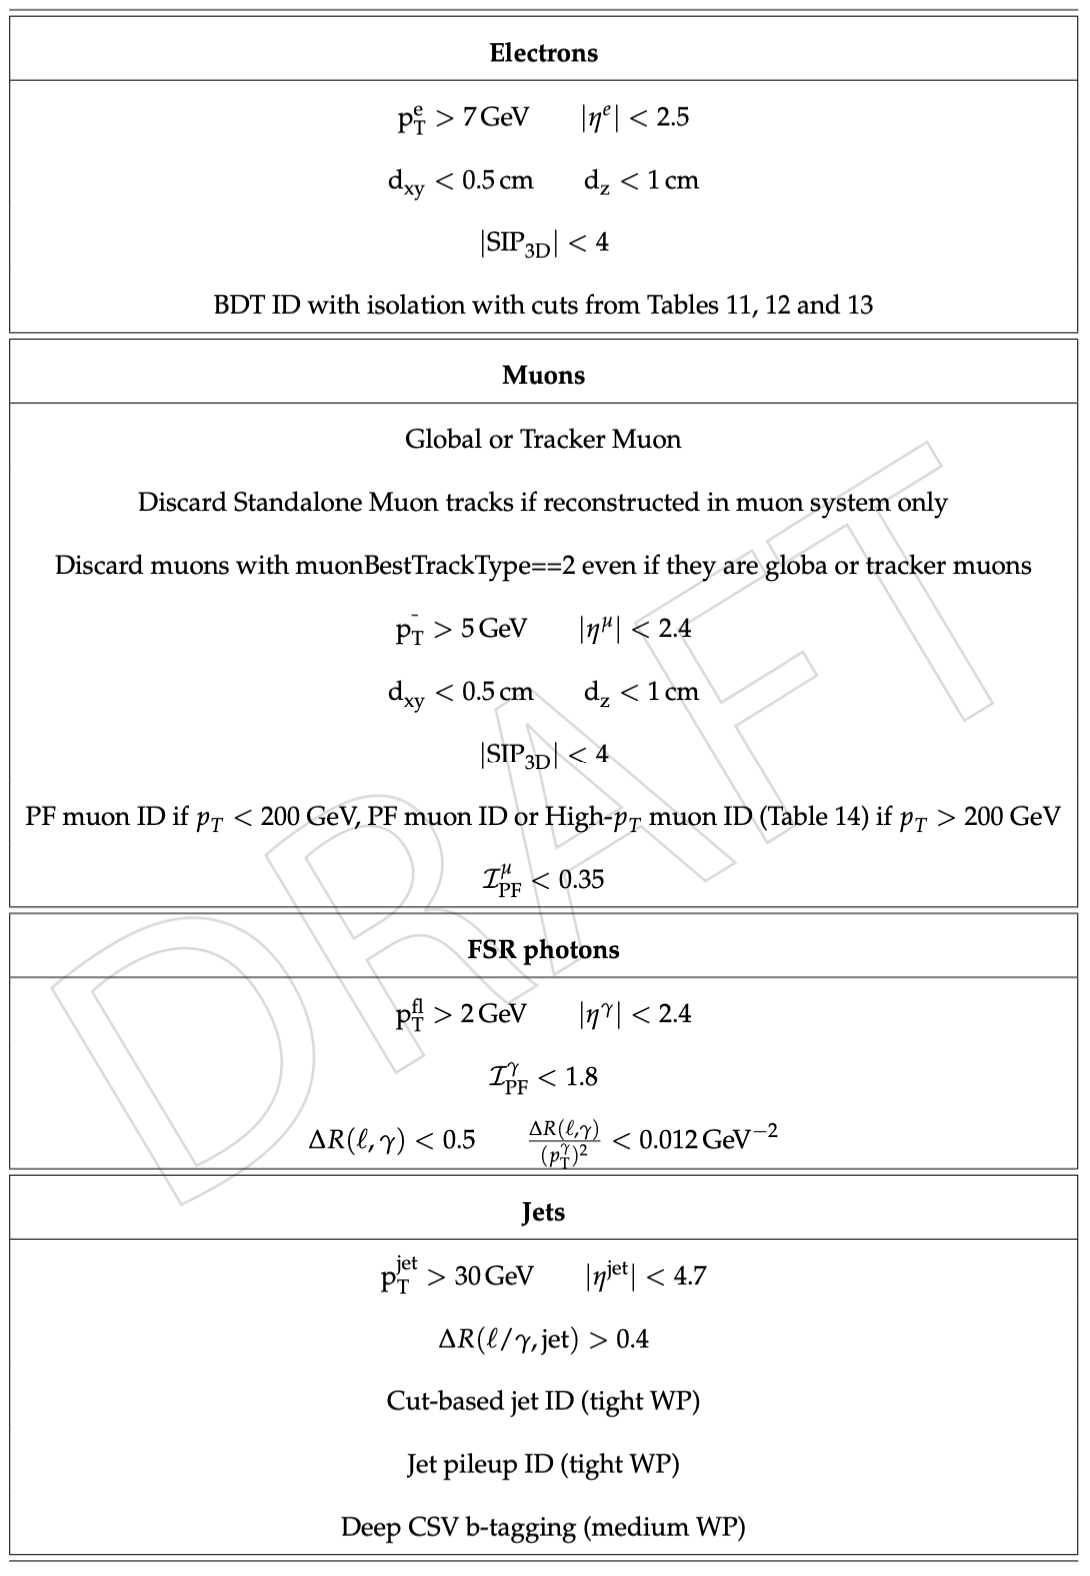
\includegraphics[height=20cm]{figures/higgsmassmeas/table_objsel_hzz4l.png}
% % 		\caption
% % 			[Branching ratios of Higgs boson decays as a function of the Higgs boson mass.]
% % 			{
% %             The branching ratios of various Higgs boson decays as a function of the Higgs boson mass
% %             over a wide range (Left) and a narrow range (Right) of values.
% %             }
% % 		\label{fig:objsel}
% % 	\end{center}
% % \end{figure}

% \subsection{\ZZ Candidate Selection}
If an event contains more than one \ZZ candidate that passes the selection criteria, then the candidate with the highest value of \Dkinbkg is selected as the overall \ZZ candidate for the event.
% % \subsection{\mathbf{\ZZ} Candidate Selection}
% % \subsection{\boldmath{\ZZ} Candidate Selection}
% % \subsection{\ZZ Candidate Selection}
% \label{sec:zz_sel}
% Words.

After the full analysis selection is implemented in each of the \fourl final states,
the expected and observed yields for the signal and background processes are given in Tables~\ref{tab:yield_sr_105to140} and~\ref{tab:yield_sr_70to170},
which count events within the narrow signal region $\left(105 < \mfourl < 140\GeV\right)$ and wide signal region $\left(70 < \mfourl < 170\GeV\right)$, respectively.
%=== Filippo is waiting to put cutflow table here. ===%
\begin{table}[!htb]
    \centering
    % \captionsetup{justification=centering}
    \topcaption
        [Yields in the narrow signal region $105 < \mfourl < 140\GeV$]
        {Number of expected and observed yields of signal and background processes within the narrow signal region $105 < \mfourl < 140\GeV$ after the full event selection using \lumiruntwo, split into the four final states.}
    \begin{tabular}{lrrrrr}
        \hline
    Process                                 & \fourmu   & \foure    & \twoetwomu    & \twomutwoe    & Inclusive    \\
        \hline
    \qqzzfourl                              &   88.8    &   38.5    & 63.7          &   41.8        &   232.8   \\
    \ggzzfourl                              &   9.7     &   4.8     & 4.8           &   3.7         &   23.0    \\
    RB                                      &   32.4    &   12.2    & 29.2          &  18.6         &   92.4    \\
    Sum of Background                       &   130.9   &   55.5    & 97.7          & 64.1          &   348.2   \\
        \hline
    Signal $\left( \mH = 125\GeV \right)$   &   90.5    &   48.2    & 64.6          & 53.0          &   256.3   \\
        \hline
    Total Expected                          &   221.4   & 103.7     & 162.3         & 117.1         &   604.5   \\
        \hline
    Total Observed                          &   ---       &   ---       &   ---           &   ---           &   ---           \\
        \hline
    \end{tabular}
    \label{tab:yield_sr_105to140}
\end{table}
\begin{table}[!htb]
    \centering
    % \captionsetup{justification=centering}
    \topcaption
        [Yields in the wide signal region $70 < \mfourl < 170\GeV$]
        {Number of expected and observed yields of signal and background processes within the wide signal region $70 < \mfourl < 170\GeV$ after the full event selection using \lumiruntwo, split into the four final states.}
    % \begin{tabular}{llllll}
    \begin{tabular}{lrrrrr}
        \hline
    Process                                 &   \fourmu &   \foure  &   \twoetwomu  &   \twomutwoe  &   Inclusive   \\
        \hline
    \qqzzfourl                              &   486.7   &   192.0   &   246.0       &   170.1       &   1094.9      \\
    \ggzzfourl                              &   29.7	&   15.2	&   13.3	    &   12.2	    &   70.5        \\
    RB                                      &   70.1    &   30.3    &	61.5        &	42.2	    &   204.1       \\
    Sum of Background                       &   586.5   &	237.5	&   320.8	    &   224.5	    &   1369.3      \\
        \hline
    Signal $\left( \mH = 125\GeV \right)$   &  92.4     &   49.6    &   66.5        &   54.3        &   262.8       \\ 
        \hline
    Total Expected                          &  679.0    &	287.2	&   387.4	    &   278.8	    &   1632.3      \\
        \hline
    Total Observed                          &   ---       &   ---       &   ---           &   ---           &   ---           \\
        \hline
    \end{tabular}
    \label{tab:yield_sr_70to170}
\end{table}

%=== TODO: Put "A" beneath first subfigure, "B" beneath second, etc.
% Reference subfigs like: ~\subref{s}
% \begin{figure}[!htb]
%     \centering
% PLOTS GO HERE
%     \begin{subfigure}{0.3\textwidth}
%         \includegraphics[width=\textwidth]{example-image}
%         \caption{First subfigure.}
%         \label{fig:first}
%     \end{subfigure}
%     \hfill
%     \begin{subfigure}{0.3\textwidth}
%         \includegraphics[width=\textwidth]{example-image}
%         \caption{Second subfigure.}
%         \label{fig:second}
%     \end{subfigure}
%     \hfill
%     \begin{subfigure}{0.3\textwidth}
%         \includegraphics[width=\textwidth]{example-image}
%         \caption{Third subfigure.}
%         \label{fig:third}
%     \end{subfigure}
            
%     \caption{Subreferences in \LaTeX.}
%     \label{fig:figures}
%     \end{figure}

% \begin{figure}[!htb]
%     \centering
%     % width=0.48\textwidth
%     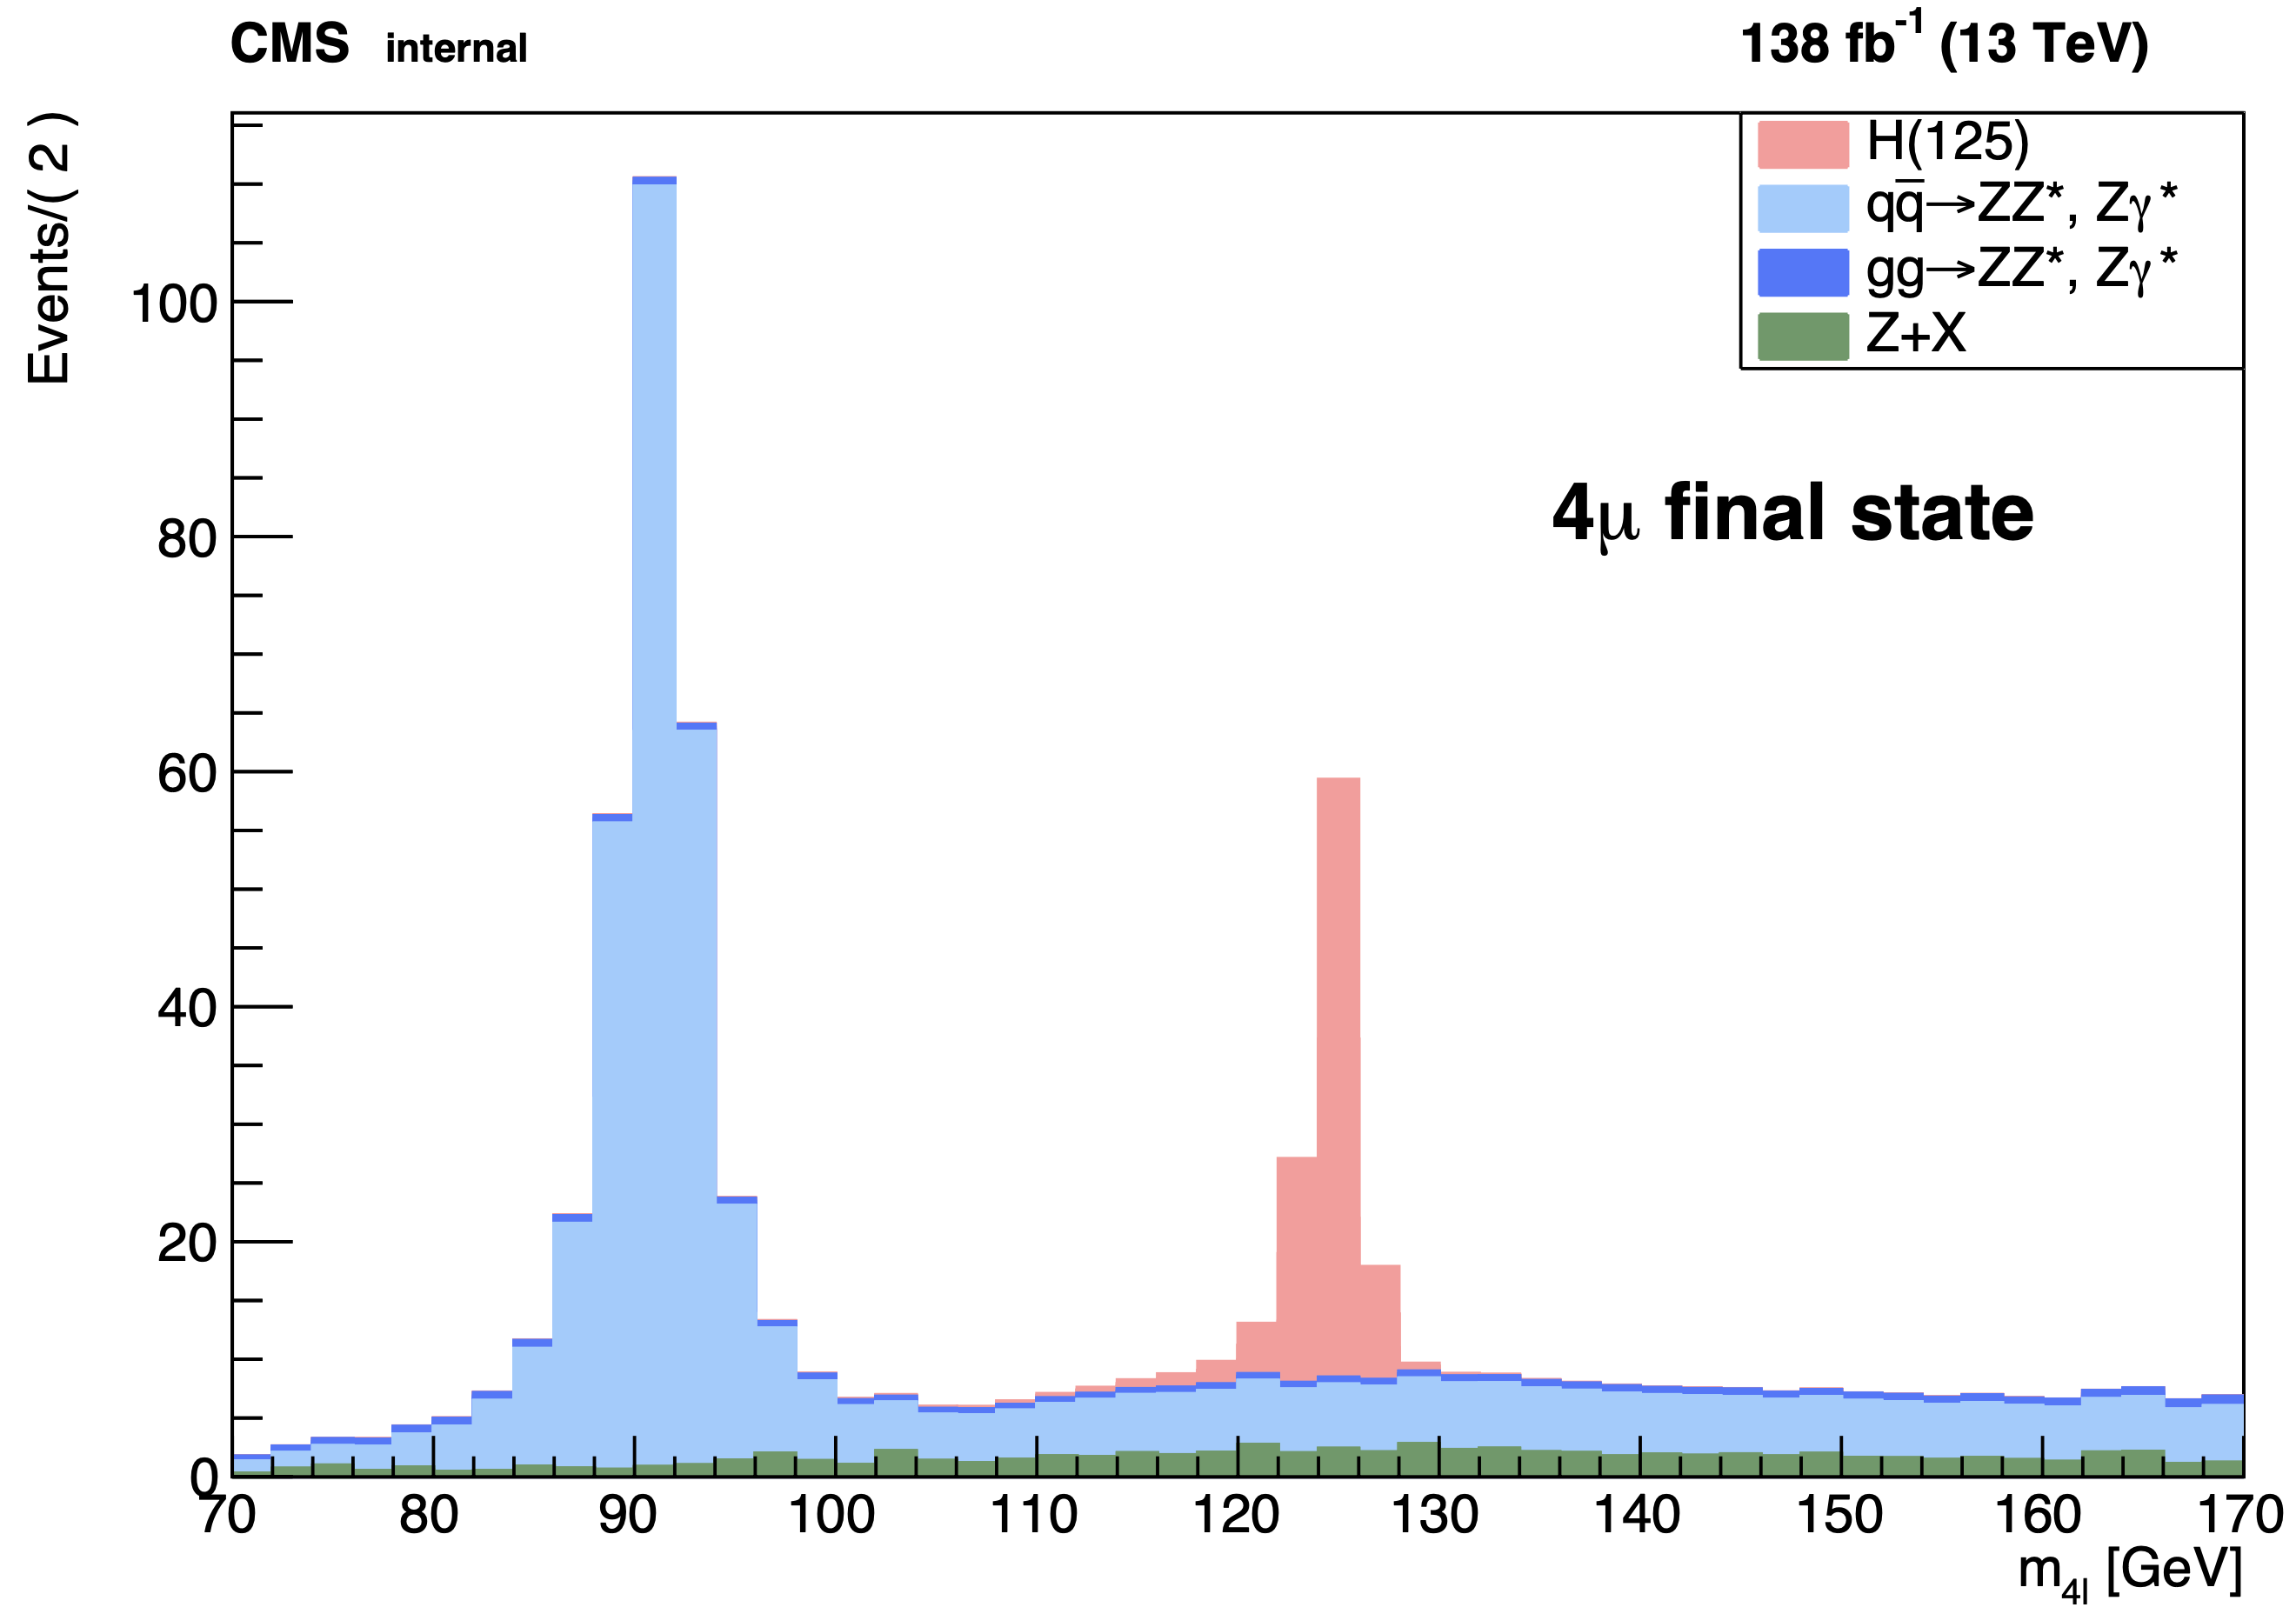
\includegraphics[height=5.5cm]{figures/higgsmassmeas/dist_m4l_allyears_fullsel_fs_4mu.png}
%     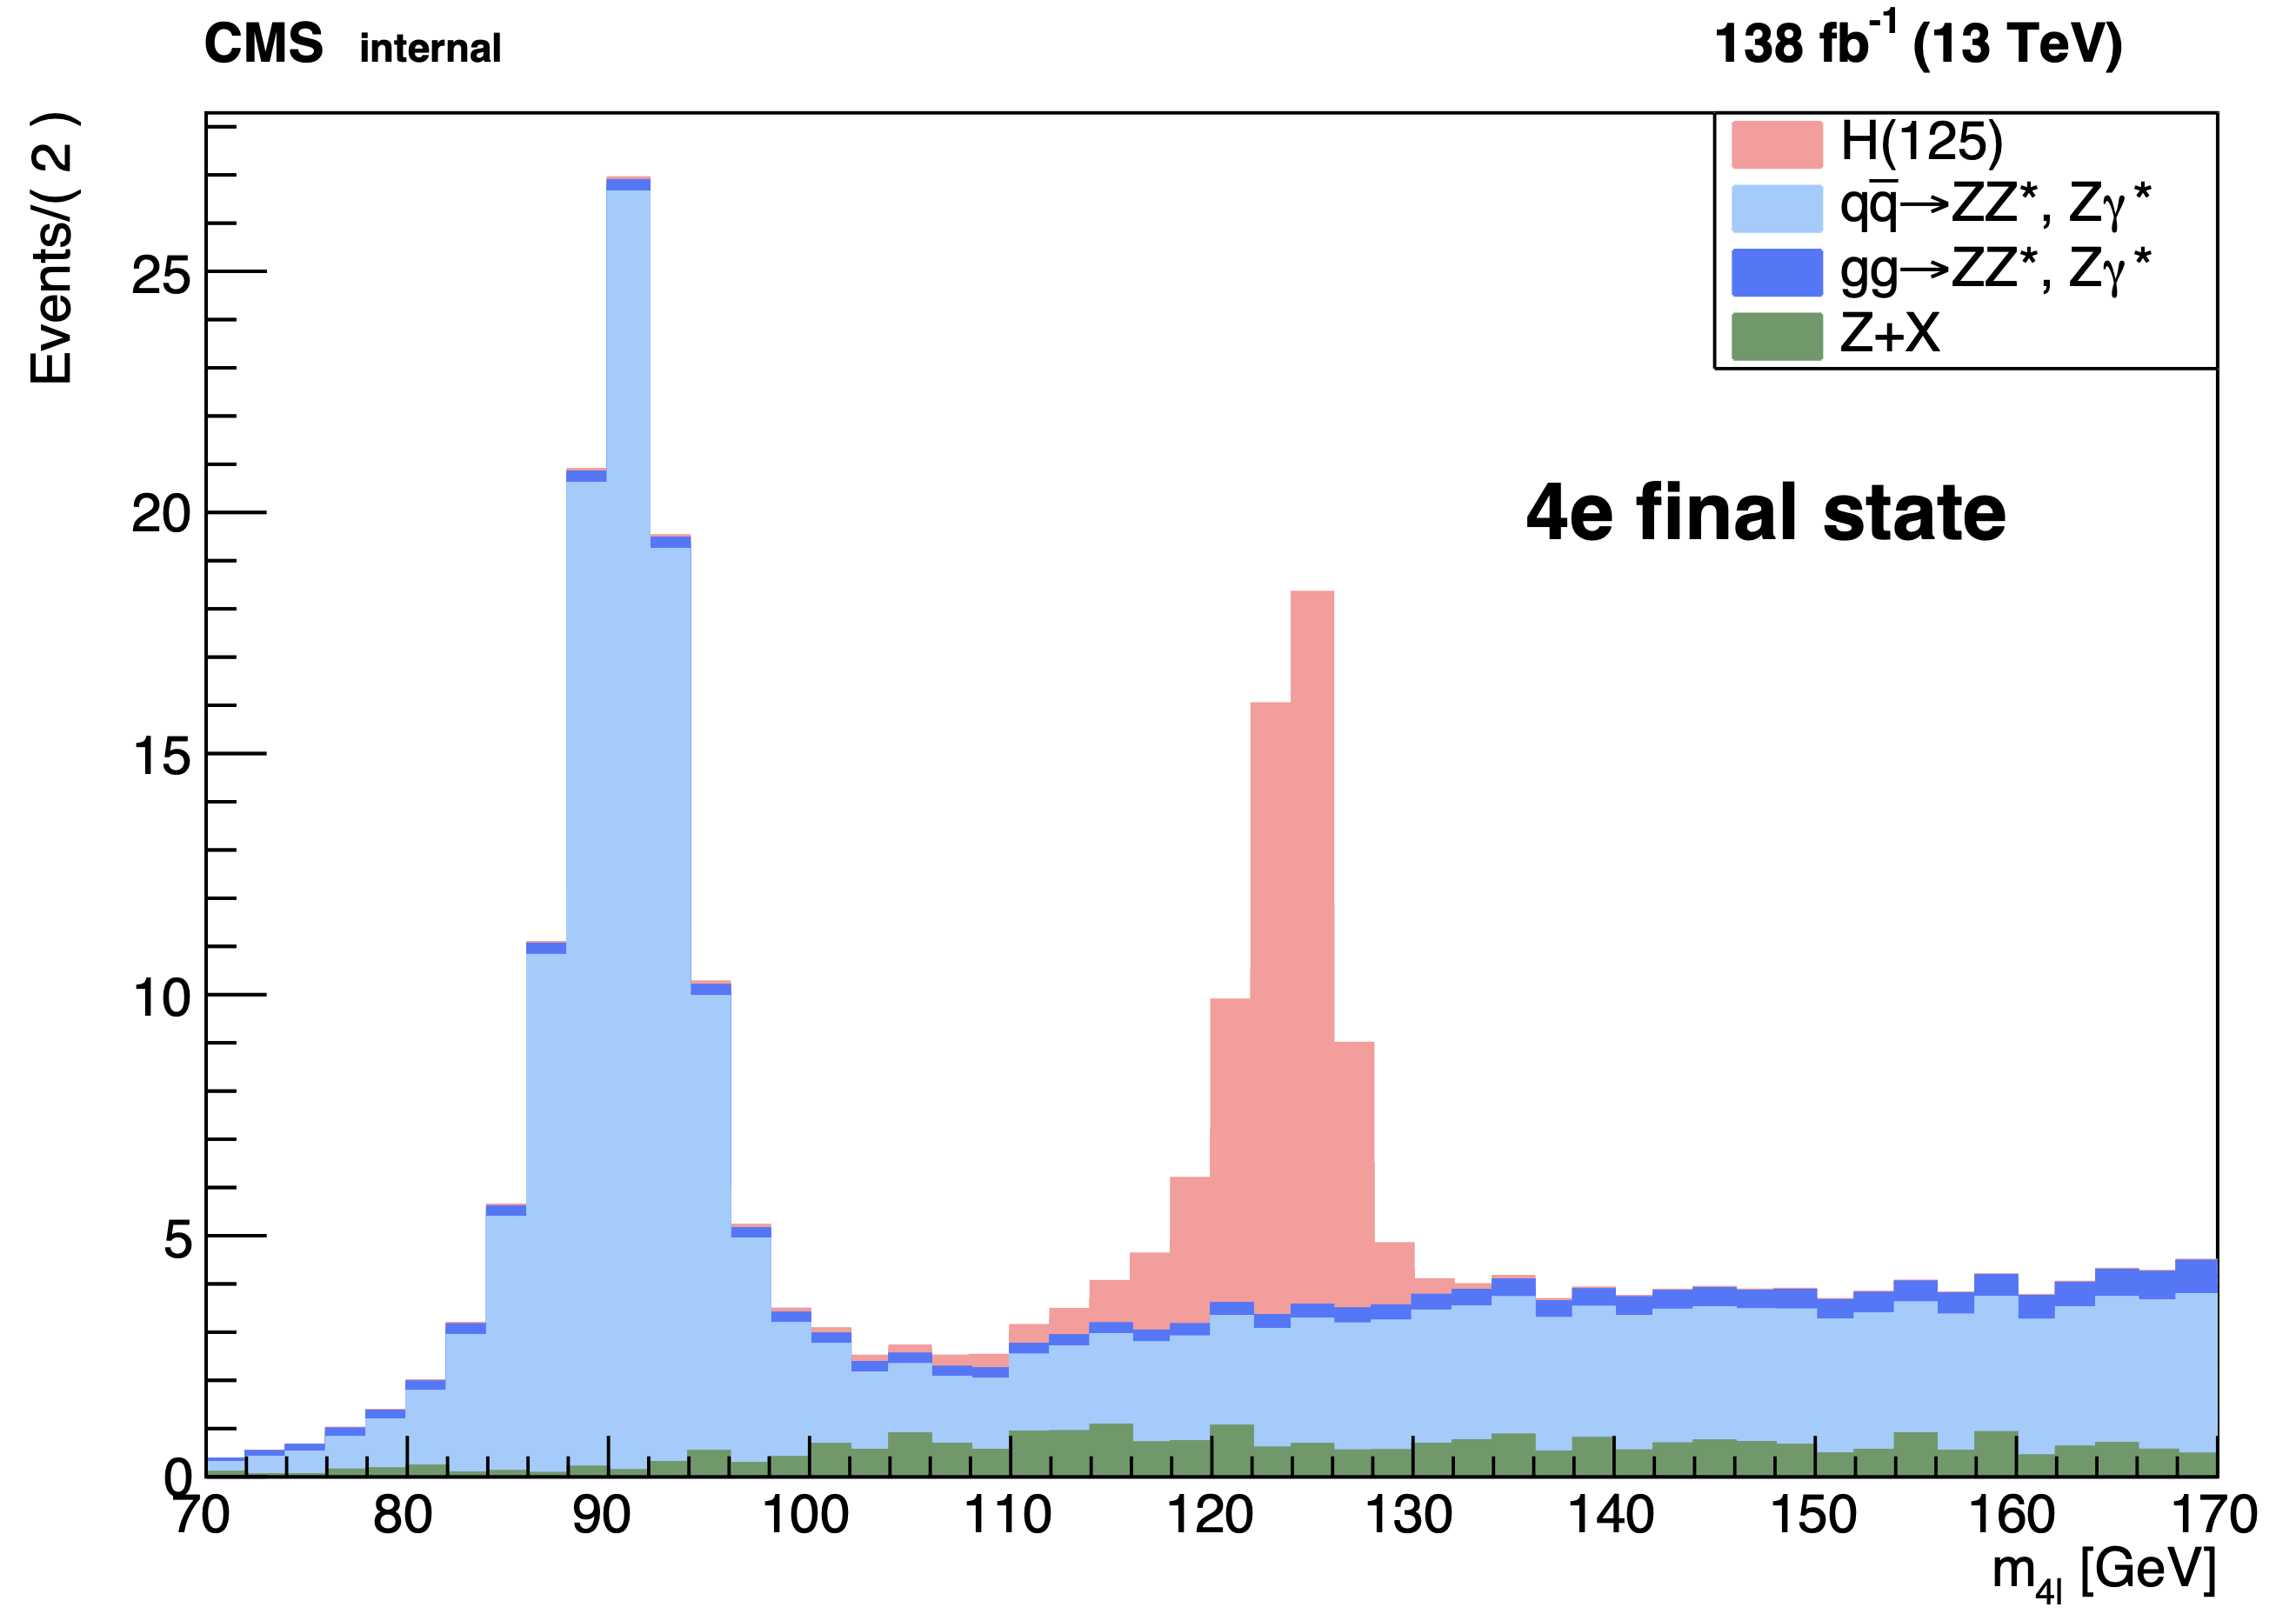
\includegraphics[height=5.5cm]{figures/higgsmassmeas/dist_m4l_allyears_fullsel_fs_4e.png}
%     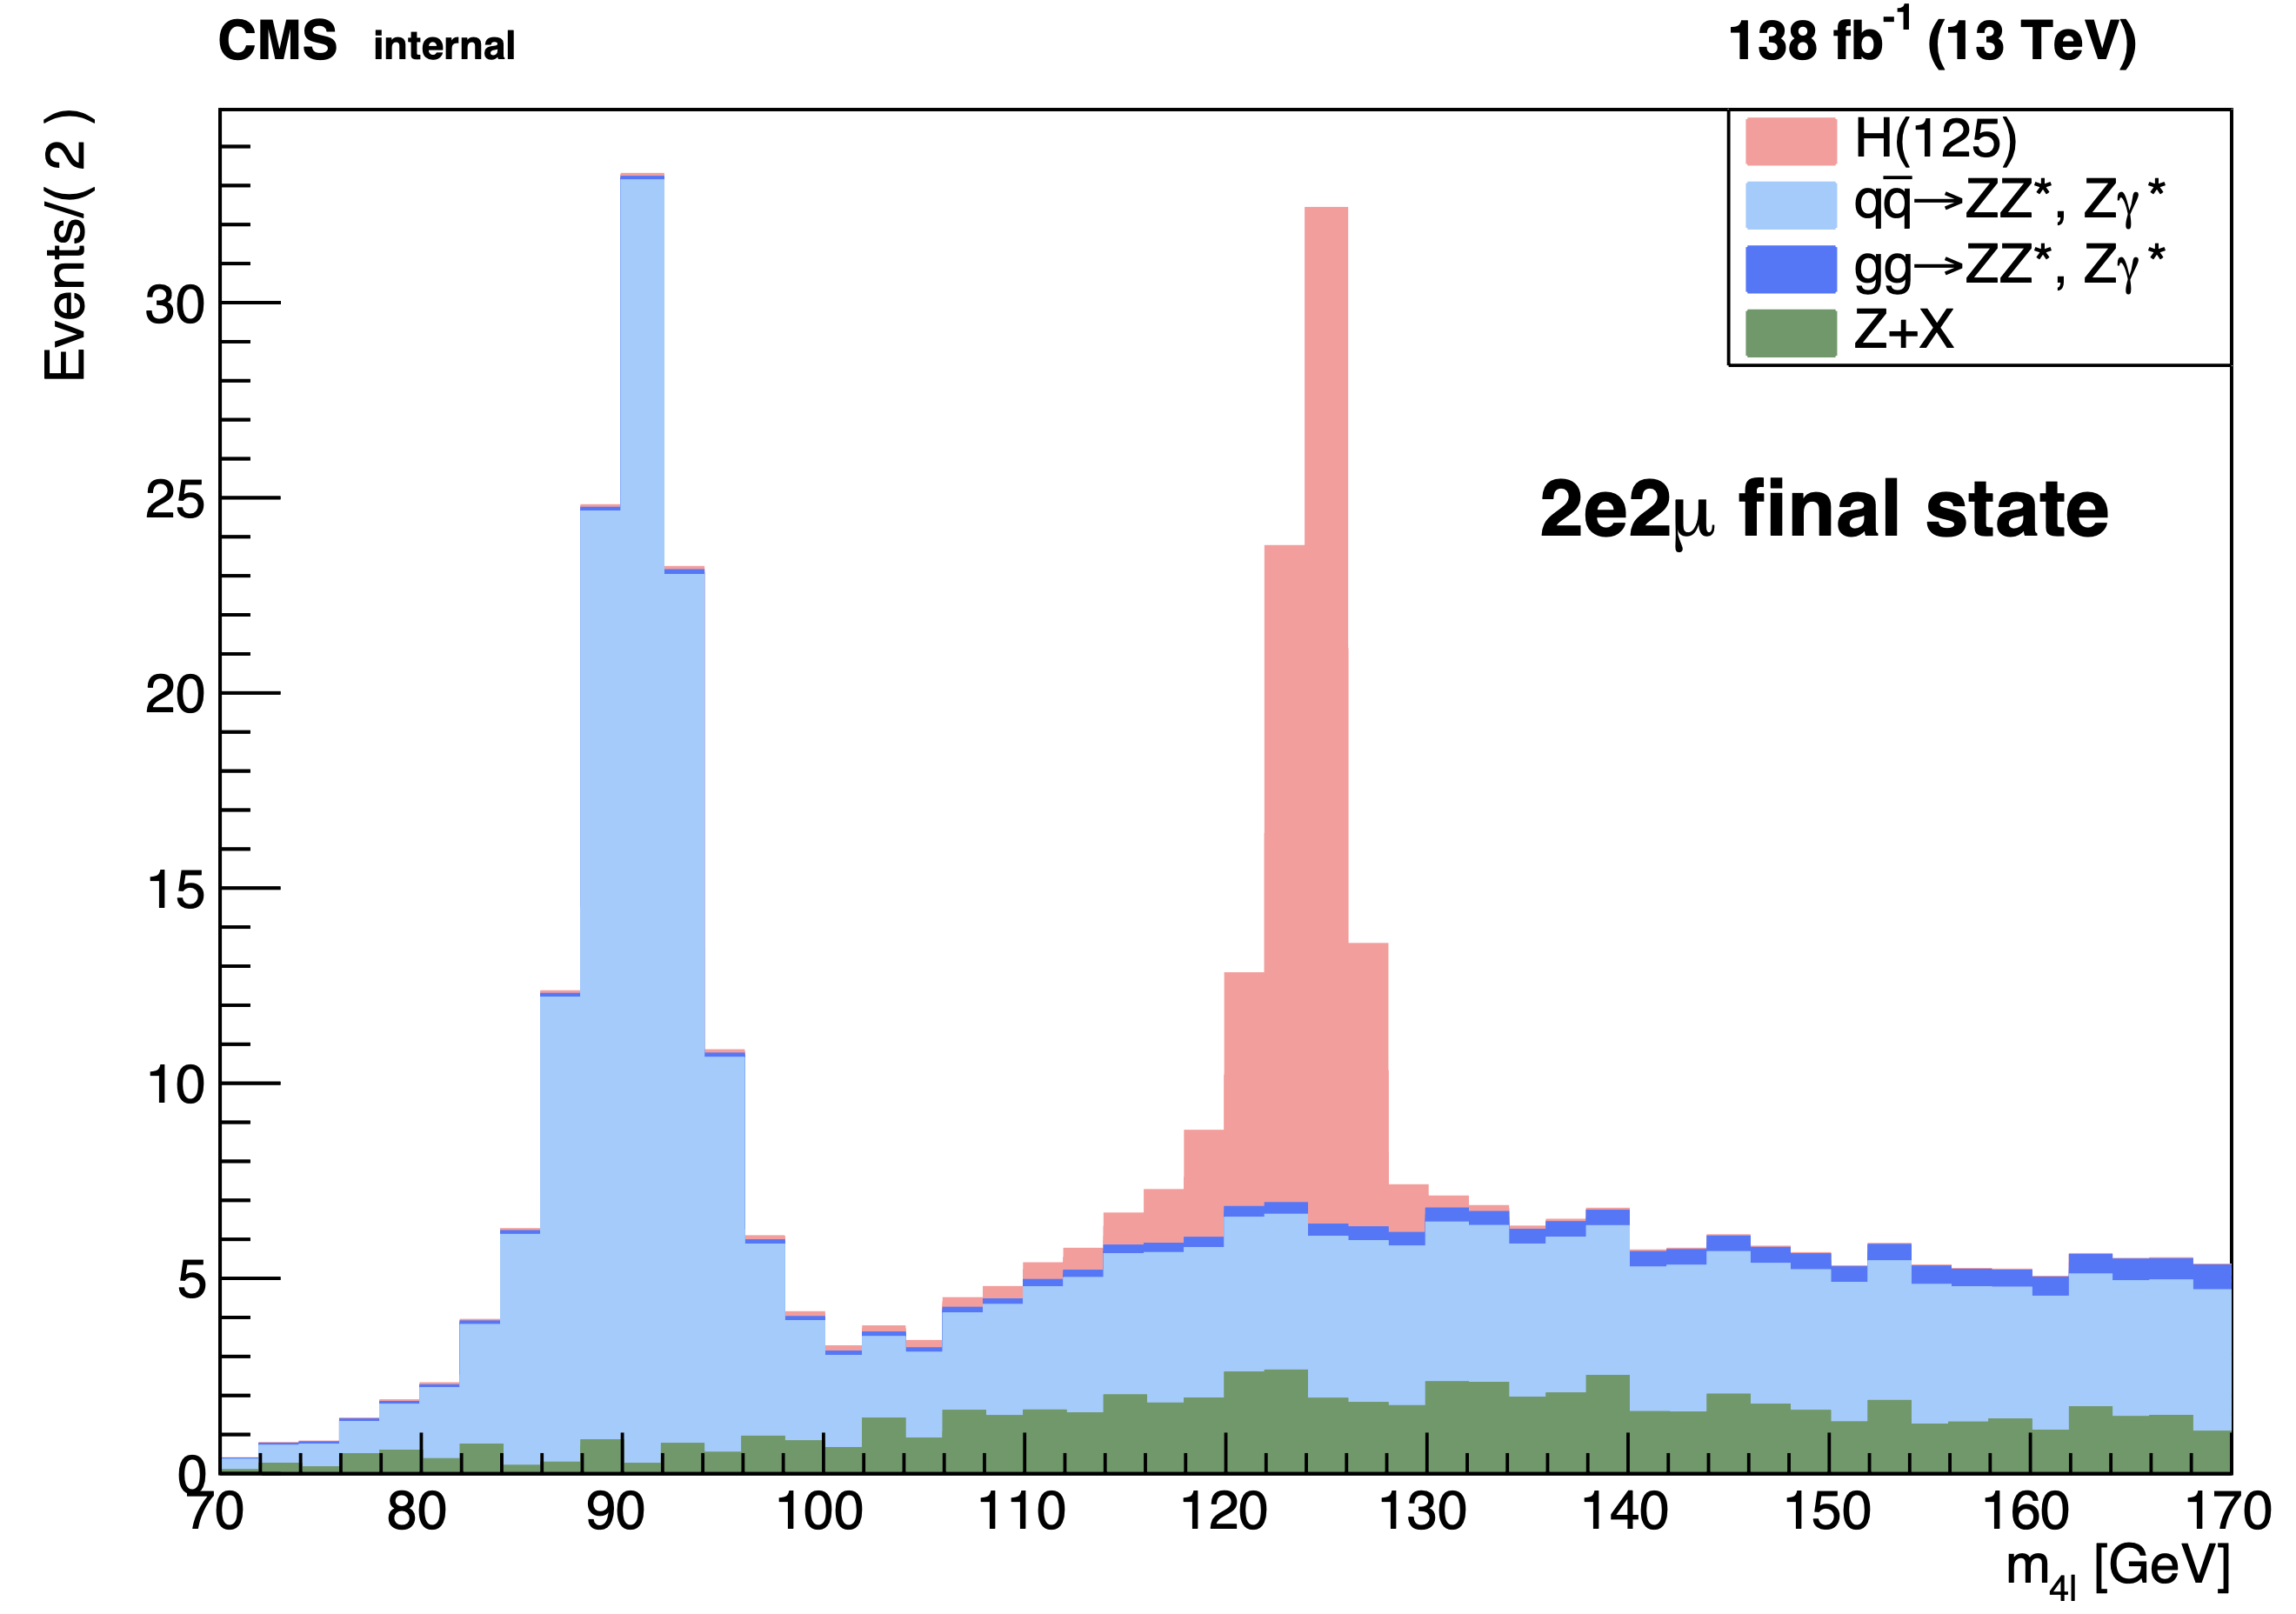
\includegraphics[height=5.5cm]{figures/higgsmassmeas/dist_m4l_allyears_fullsel_fs_2e2mu.png}
%     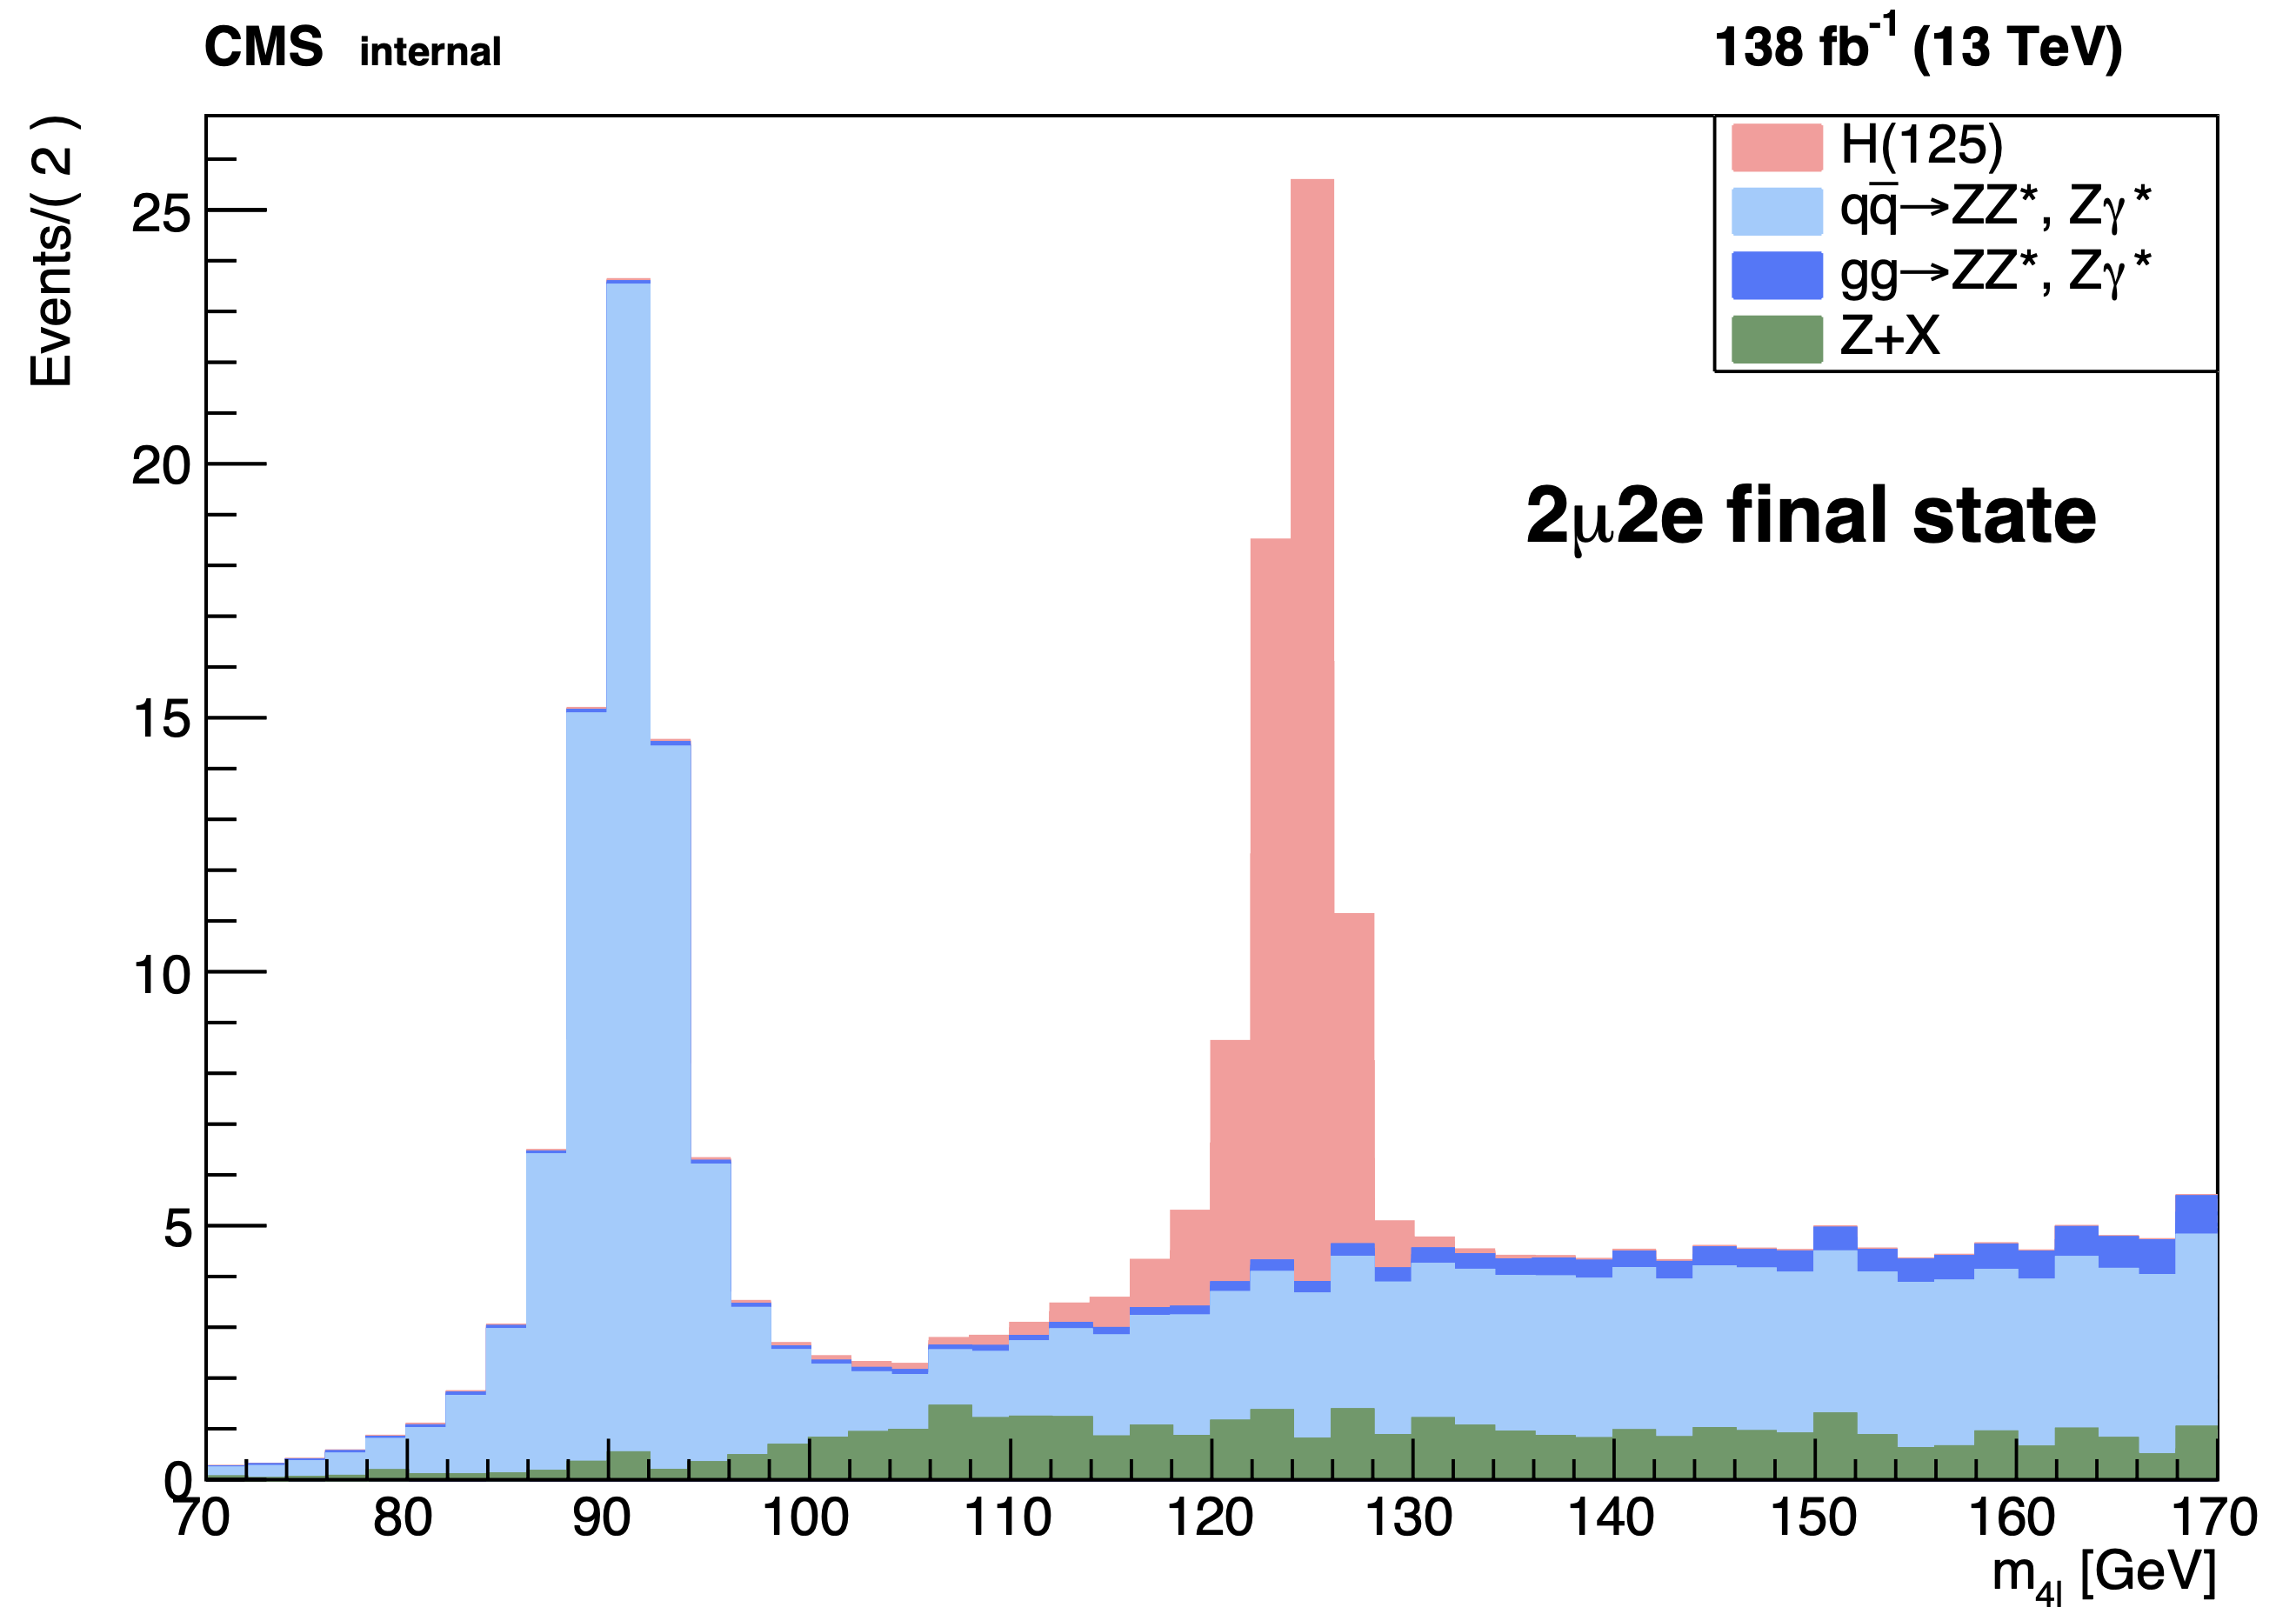
\includegraphics[height=5.5cm]{figures/higgsmassmeas/dist_m4l_allyears_fullsel_fs_2mu2e.png}
%     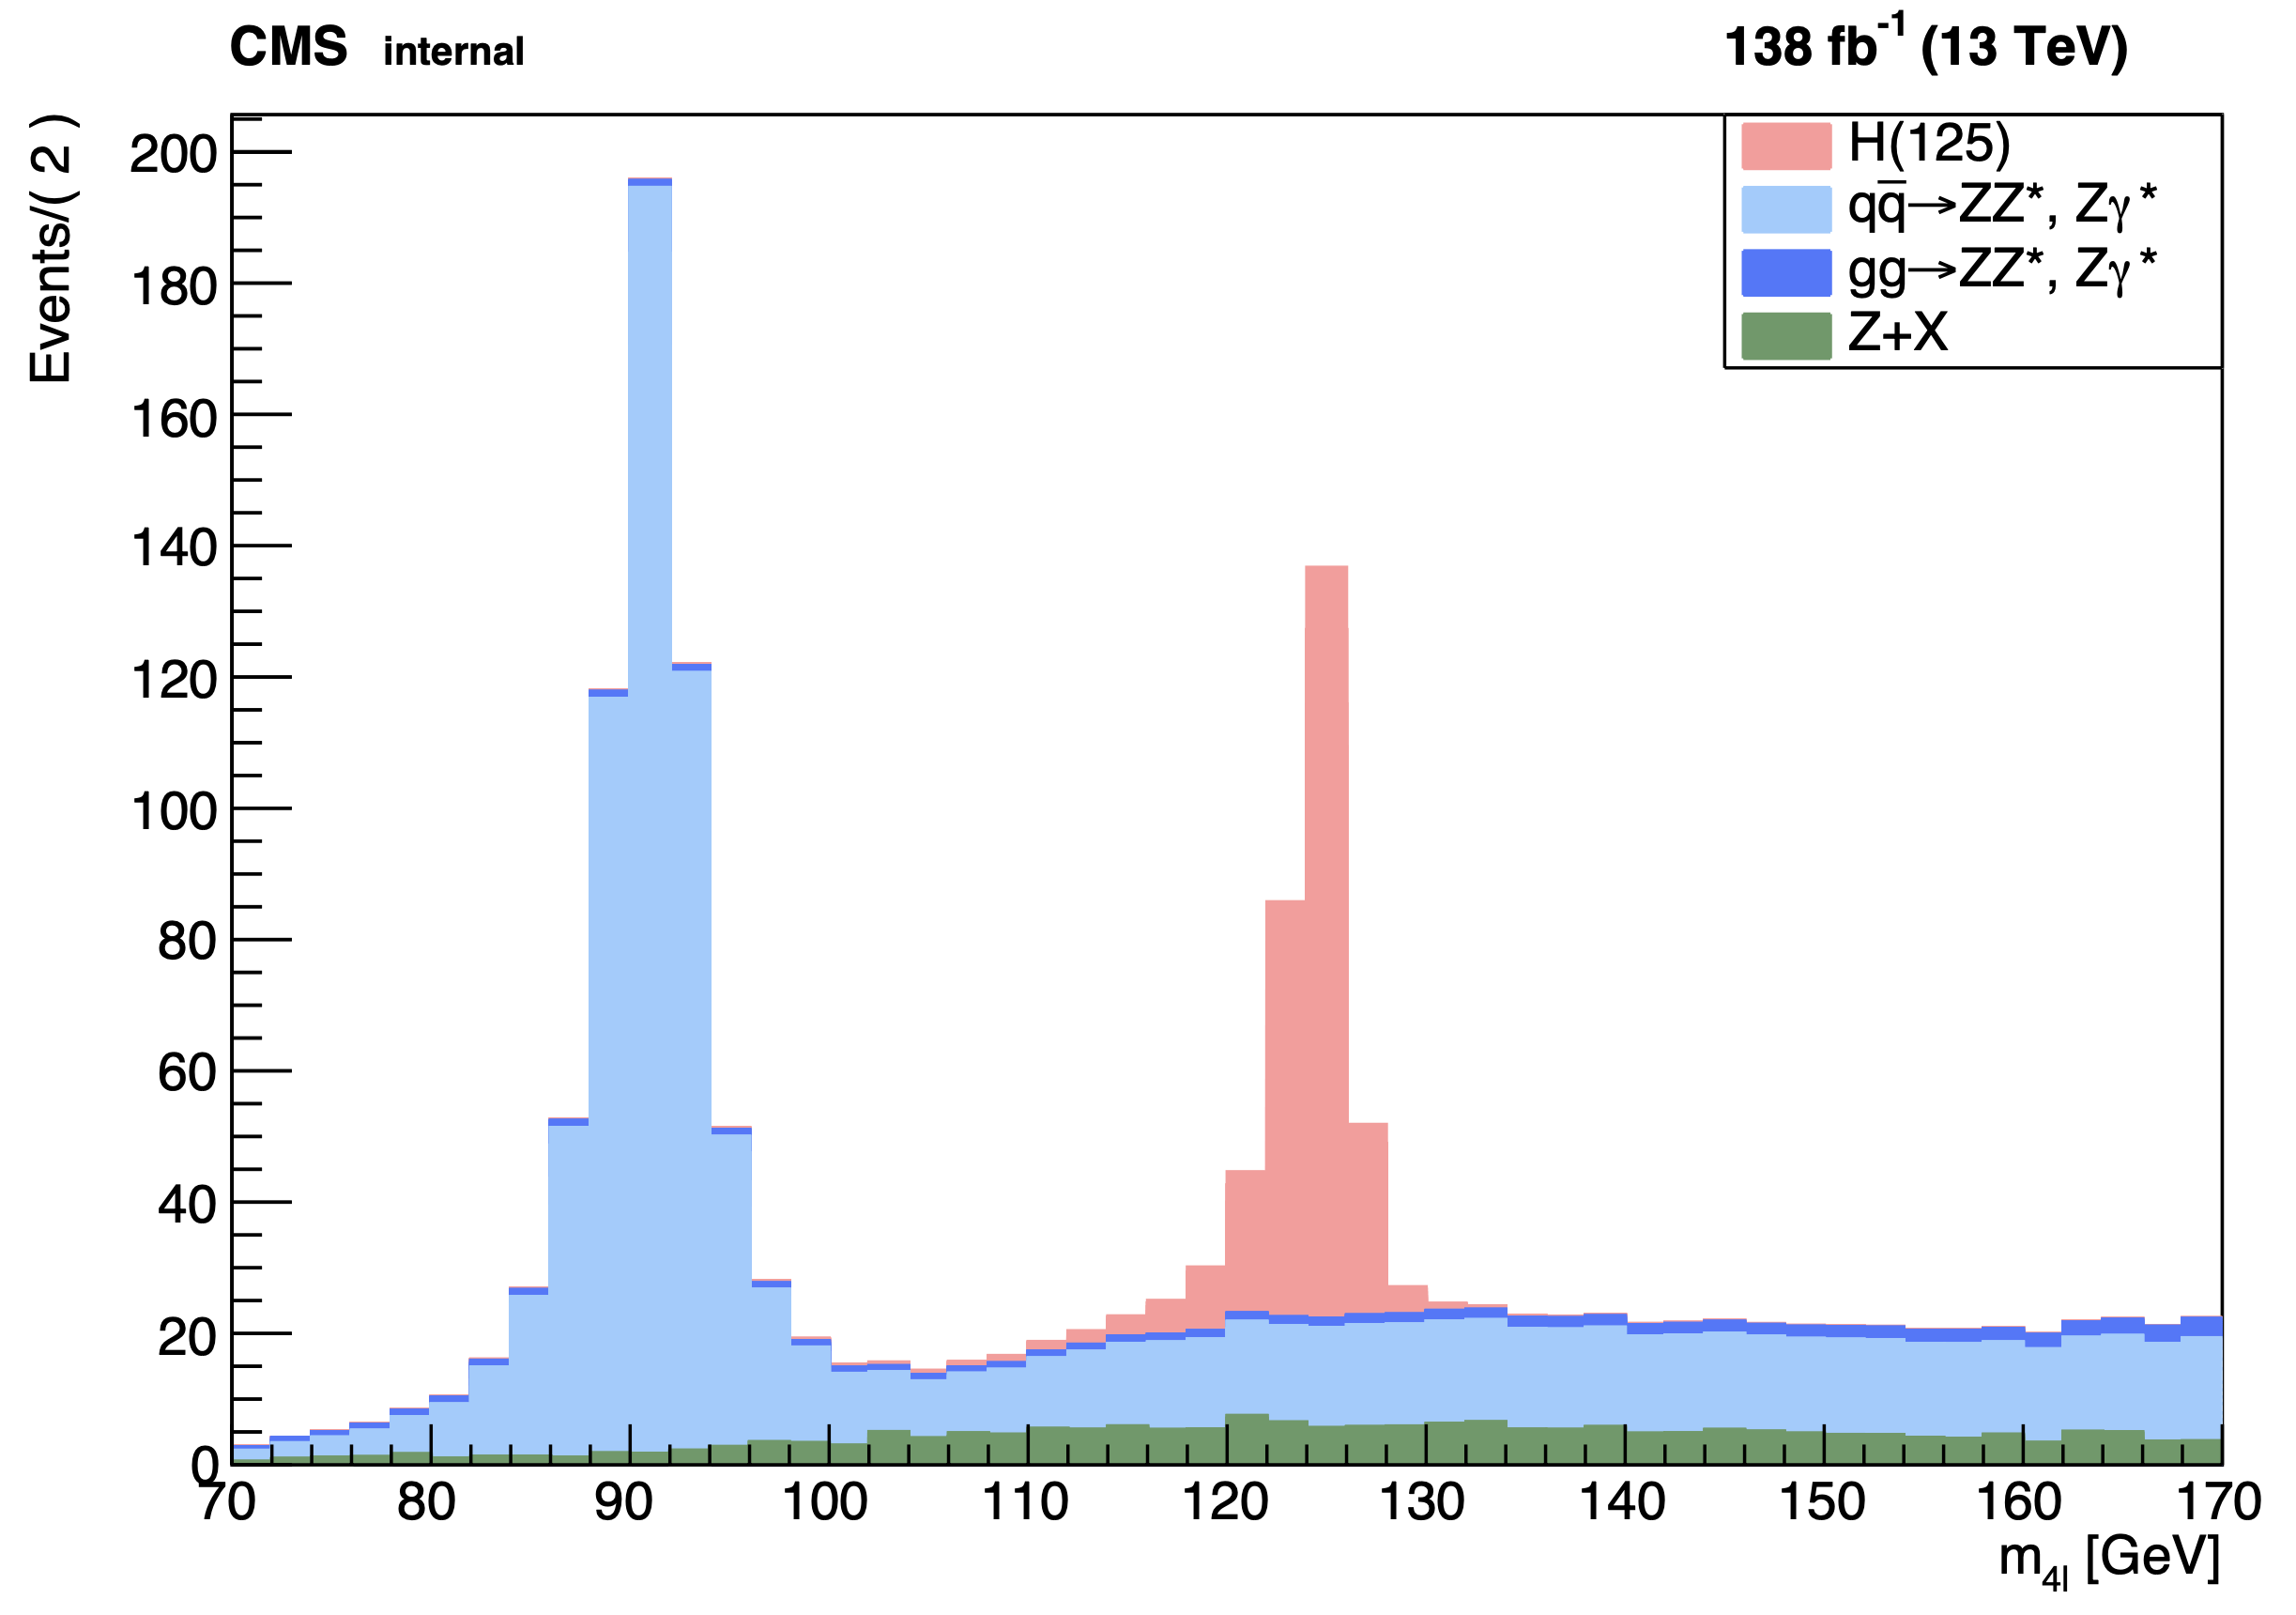
\includegraphics[height=7.0cm]{figures/higgsmassmeas/dist_m4l_allyears_fullsel_fs_inclus.png}
%     \caption
%         [Some words here.]
%         {Distribution of the four-lepton invariant mass for each final state. A) blah blah}
%     \label{fig:dist_m4l_fullsel}
% \end{figure}

\begin{multiFigure}
    \centering
    \addFigure{0.48}{figures/higgsmassmeas/dist_m4l_allyears_fullsel_fs_4mu.png}
    \addFigure{0.48}{figures/higgsmassmeas/dist_m4l_allyears_fullsel_fs_4e.png}
    \addFigure{0.48}{figures/higgsmassmeas/dist_m4l_allyears_fullsel_fs_2e2mu.png}
    \addFigure{0.48}{figures/higgsmassmeas/dist_m4l_allyears_fullsel_fs_2mu2e.png}
    \addFigure{0.60}{figures/higgsmassmeas/dist_m4l_allyears_fullsel_fs_inclus.png}
    % \addFigure[Z]{0.6}{./theworld.png}  % <== Control the label.
    \captionof{figure}  % Type of caption.
        [Distribution of the four-lepton invariant mass for each final state.]
        {Distribution of the four-lepton invariant mass for each final state.}
\end{multiFigure}
